\section{Experiments and Results}

\subsection{DME Staging}
\gls{dme} staging from color fundus images involves grading images on a scale from 0 to 2, with 0 being healthy and 2 being severe (see Fig.~\ref{fig:dme}). Differentiation between the grades relies on the presence of hard exudates present in different locations of the retina. Specifically, a grade of 0 implies that no hard exudates are present at all, a grade of 1 implies that hard exudates are located in the retina periphery (\ie,~outside a circular region centered at the fovea center with radius of one optic disc diameter), and a grade of 2 when hard exudates are in the macular region~\cite{ren2018diabetic}.
\begin{figure}[b!]
\begin{center}
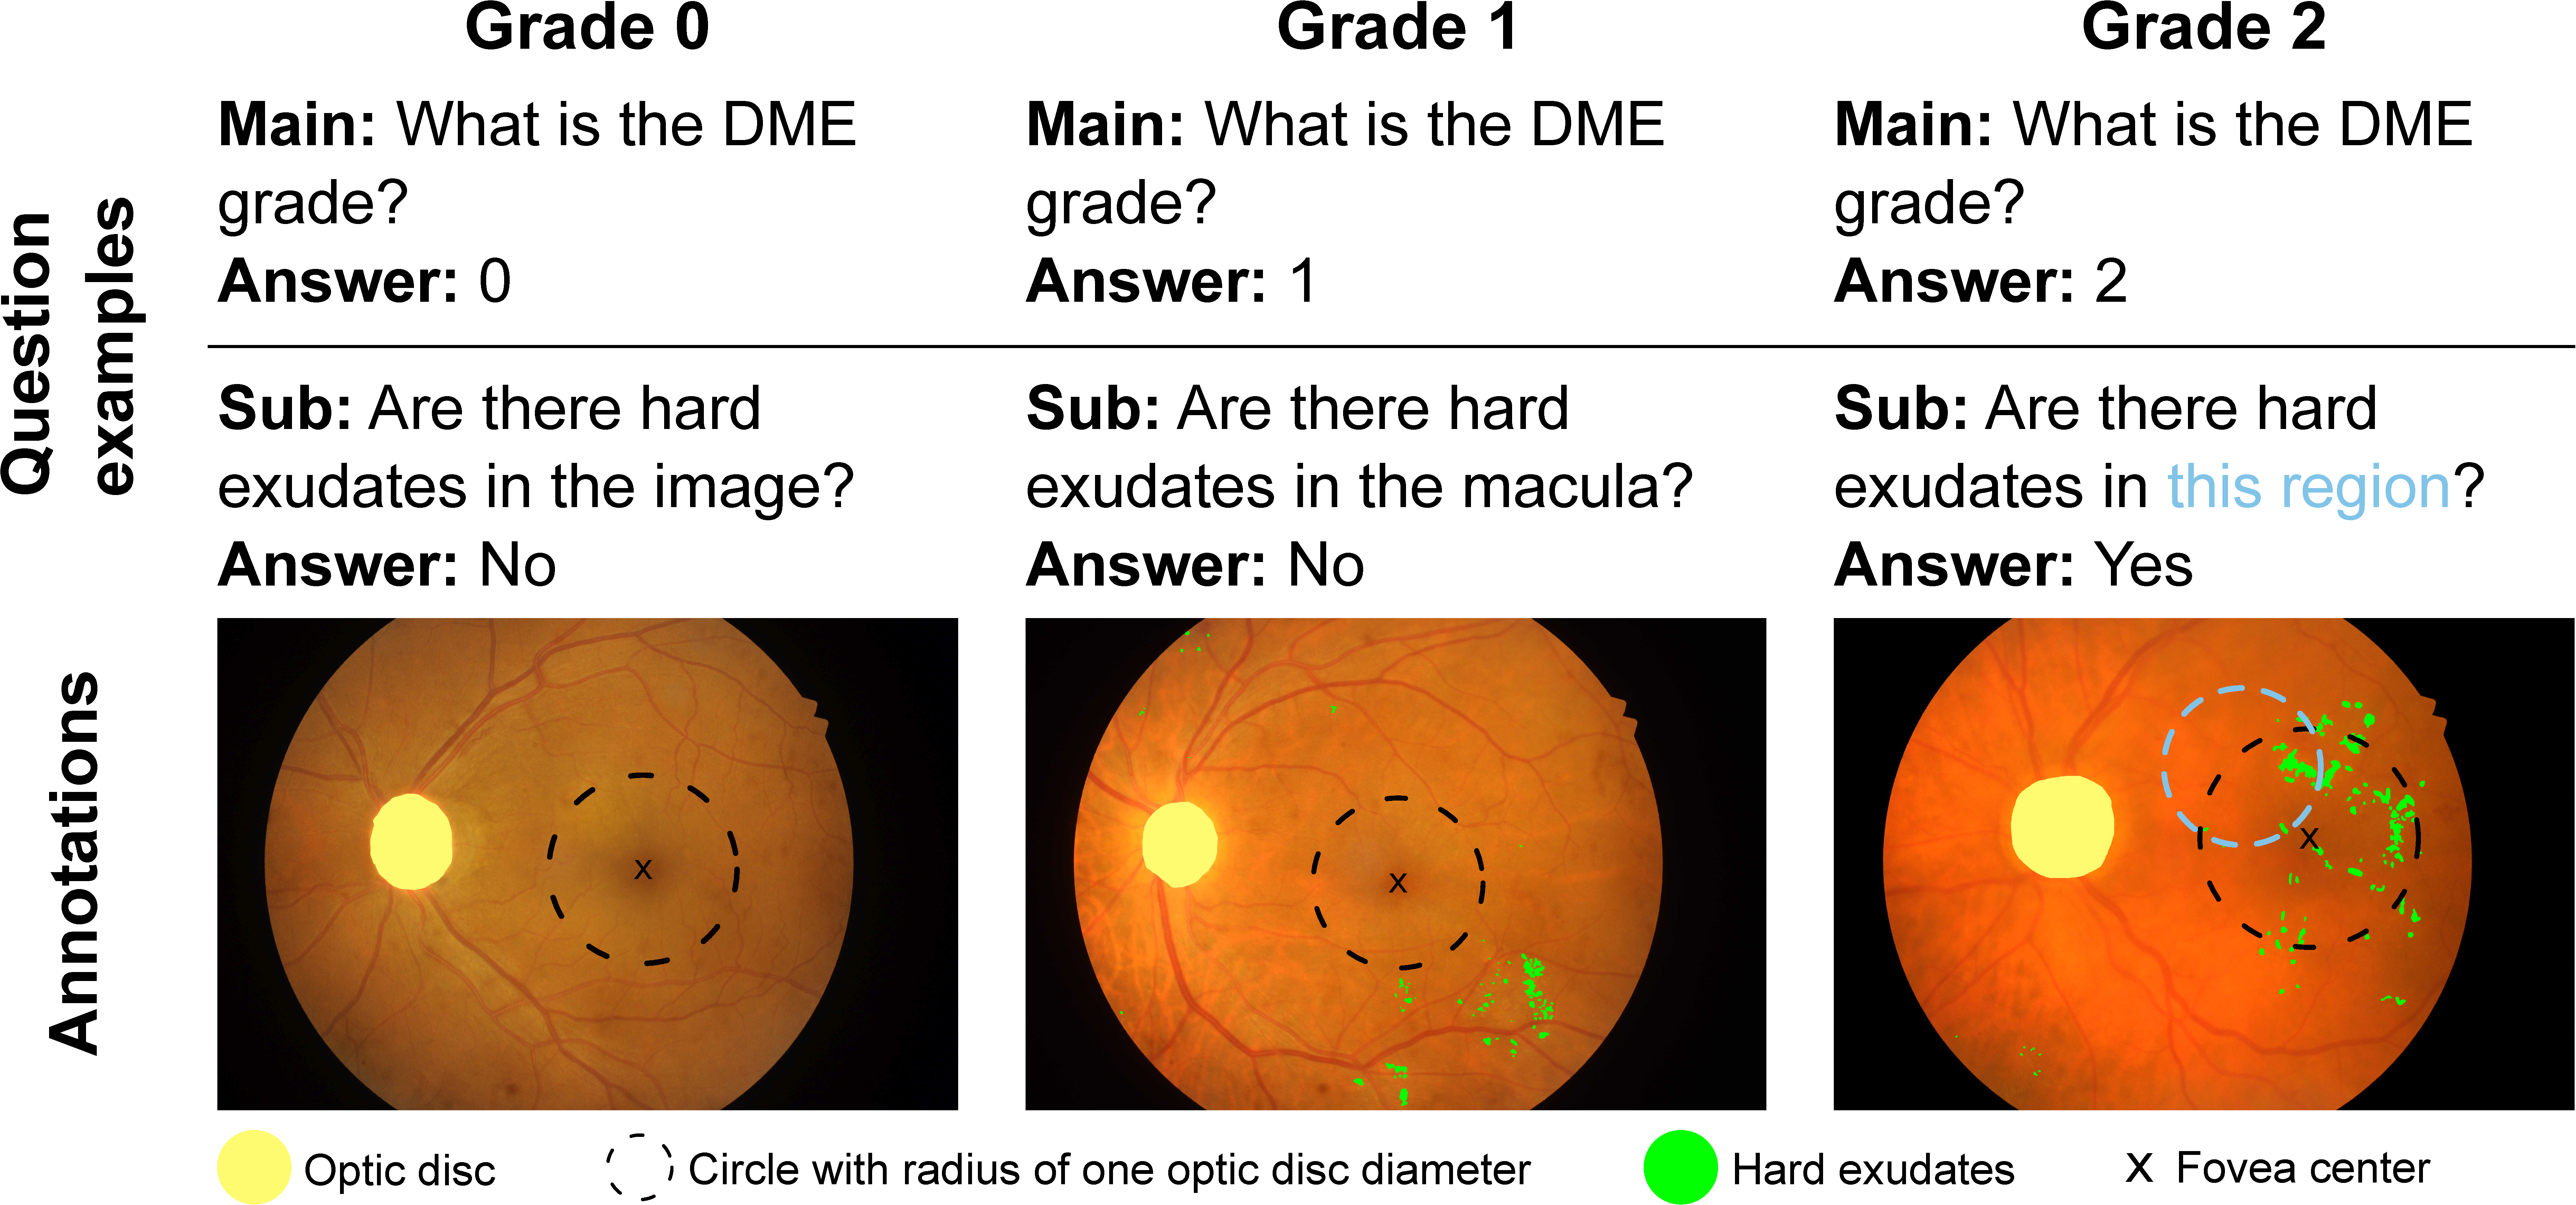
\includegraphics[width=0.9\textwidth]{Figures/Part2_Consist/01_mainsub/dme_2.pdf}
\caption{DME risk grading. Grade 0 is assigned if there are no hard exudates present in the whole image. Grade 1 is assigned if there are hard exudates, but only located outside a circle centered at the fovea with radius of one optic disc diameter. Grade 2 is assigned if there are hard exudates located within the circle. Examples of main and sub-questions are provided for each grade.}
\label{fig:dme}
\end{center}
\end{figure}

\subsection{Dataset}
To validate our method, we make use of two publicly available datasets: the Indian Diabetic Retinopathy Image Dataset (IDRiD)~\cite{idrid} and the e-Ophta dataset~\cite{decenciere2013teleophta}. From the IDRiD dataset, we use images from the segmentation and grading tasks, which consist of 81 and 516 images, respectively. Images from the segmentation task include segmentation masks for hard exudates and images from the grading task only have the \gls{dme} grade. On the other hand, the e-Ophta dataset comprises 47 images with segmentation of hard exudates and 35 images without lesions. Combining both datasets yields a dataset of 128 images with segmentation masks for hard exudates and 128 images without any lesions, plus 423 images for which only the \gls{dme} risk grade is available. 

In this context, we consider main questions to be those asking ``What is the \gls{dme} risk grade?" when considering the entire image. Sub-questions were then defined as questions asking about the presence of the hard exudates. For instance, as shown in Fig.~\ref{fig:dme}{(Right)}, ``Are there hard exudates in this region?" where the region designated contains the macula. In practice, we set three types of sub-questions: ``are there hard exudates in this image?", ``are there hard exudates in the macula?" and ``are there hard exudates in this region?". We refer to these three questions as \textit{whole}, \textit{macula} and \textit{region} questions, respectively. For the region sub-questions, we consider circular regions that can be centered anywhere, or centered on the fovea, depending on availability of fovea center location annotations. As mentioned in Sec.~\ref{sec:mainsub_method}, to answer questions about regions, images are masked so that only the region is visible.

The total number of question-answer pairs in our dataset consists of 9779 for training {(4.4\% main, 21.4\% sub, 74.2\% ind)}, 2380 for validation {(4.5\% main, 19.2\% sub, 76.3\% ind)} and 1311 for testing {(10\% main, 46.1\% sub, 43.9\% ind)}, with images in the train, validation and test sets being mutually exclusive.

\subsection{Experimental Setup}

We compare our approach to a baseline model that does not use the proposed $\ell_{\textrm{cons}}$ loss, equivalent to setting $\lambda=0$. In addition, we compare our method against the attention-matching method, SQuINT~\cite{selvaraju2020squinting}, as it is a state-of-the-art alternative to our approach that can be used with the same \gls{vqa} model architecture.

Our \gls{vqa} model uses an ImageNet-pretrained ResNet101~\cite{he2016deep} with input image of $448\times 448$~pixels and an embedding of 2048~dimensions for the image encoding. For text encoding, a single-layer \gls{lstm}~\cite{hochreiter1997long} network processes the input question with word encoding of length 300 and produces a single question embedding of 1024~dimensions. The multi-glimpse attention mechanism~\cite{xu2015show} uses 2~glimpses and dropout rate~$0.25$, and the multimodal fusion stage uses standard concatenation. The final classifier is a multi-layer perceptron with hidden layer of 1024 dimensions and dropout rate of 0.25. Hyperparameters~$\lambda$ and~$\gamma$ were empirically adjusted to 0.5 and~1.0, respectively. 

All experiments were implemented using PyTorch~1.10.1 and run on a Linux machine with an NVIDIA RTX 3090 graphic card using 16~GB of memory and 4~CPU cores. All methods use the weighted cross-entropy as the base \gls{vqa} loss function. Batch size was set to~64, and we used Adam for optimization with a learning rate of $10^{-4}$. Maximum epoch number was 100 and we use early stopping policy to prevent overfitting, with patience of 20~epochs \footnote{Our code and data are available at \url{https://github.com/sergiotasconmorales/consistency_vqa}}.

We report accuracy and consistency~\cite{selvaraju2020squinting} performances, using two different definitions of consistency for comparison. Consistency, C1, is the percentage of sub-questions that are answered correctly when the main question was answered correctly. Consistency, C2, is the percentage of main questions that are answered correctly when all corresponding sub-questions were answered correctly.

\subsection{Results}
Table \ref{tab:results} shows the results.
% for the best values of the hyperparameters $\lambda$ and $\gamma$. \RS{I don't understand this. Do we have other values of $\lambda$ and $\gamma$. Do we have that as well for Squint}.
We compare these results to the case in which the value of $\lambda$ is~0, which corresponds to the baseline in which no additional loss term is used. For each case, we present the overall accuracy and the accuracy for each type of question, as well as the consistency values. Fig.~\ref{fig:examples} illustrates the performance of each method with representative qualitative examples.


\begin{table}[!t]
\begin{center}
\resizebox{\textwidth}{!}{
\begin{tabular}{llllllll}
\toprule
\multicolumn{1}{l}{\multirow{2}{*}{Case}}    &  \multicolumn{5}{c}{Accuracy} & \multicolumn{2}{c}{Consistency} \\ \cline{2-8} \multicolumn{1}{c}{}  
                   & \multicolumn{1}{l}{overall}      & \multicolumn{1}{l}{grade}        & \multicolumn{1}{l}{whole}        & \multicolumn{1}{l}{macula}       & \multicolumn{1}{l}{region}       & \multicolumn{1}{c}{C1}            & \multicolumn{1}{c}{C2}          

\\ \hline
\multicolumn{1}{l}{Baseline (no att.)}                                 & \multicolumn{1}{l}{77.54 } & \multicolumn{1}{l}{73.59} & \multicolumn{1}{l}{81.37 } & \multicolumn{1}{l}{83.37}& \multicolumn{1}{l}{76.66 } & \multicolumn{1}{l}{81.70 }  & \multicolumn{1}{l}{91.86 } 

\\ 
\multicolumn{1}{l}{Baseline (att.)}                            & \multicolumn{1}{l}{81.46 } & \multicolumn{1}{l}{80.23} & \multicolumn{1}{l}{83.13 } & \multicolumn{1}{l}{\textbf{87.18} }& \multicolumn{1}{l}{80.58 } & \multicolumn{1}{l}{89.21 }  & \multicolumn{1}{l}{96.92 } 

\\ 
\multicolumn{1}{l}{Baseline (att.) + SQuINT~\cite{selvaraju2020squinting}  }                                  & \multicolumn{1}{l}{80.58} & \multicolumn{1}{l}{77.48} & \multicolumn{1}{l}{82.82} & \multicolumn{1}{l}{85.34}& \multicolumn{1}{l}{80.02} & \multicolumn{1}{l}{88.17}  & \multicolumn{1}{l}{94.62} 

\\ 
\multicolumn{1}{l}{Baseline (att.) + Ours ($\lambda=0.5,\gamma=1$)}             & \multicolumn{1}{l}{\textbf{83.49} } & \multicolumn{1}{l}{\textbf{80.69} } & \multicolumn{1}{l}{\textbf{84.96} } & \multicolumn{1}{l}{\textbf{87.18} } & \multicolumn{1}{l}{\textbf{83.16}} & \multicolumn{1}{l}{\textbf{94.20} } & \multicolumn{1}{l}{\textbf{98.12} } 

\\ \bottomrule                  
\end{tabular}
}
\end{center}
\caption{Average test accuracy and consistency values for the different models. Results shown are averaged over 10 models trained with different seeds. Accuracy values are presented for all questions (overall), for main questions (grade) and for sub-questions (whole, macula and region). Both measures of consistency are shown as well.}
\label{tab:results}
\end{table}
\begin{figure}[!t]
\begin{center}
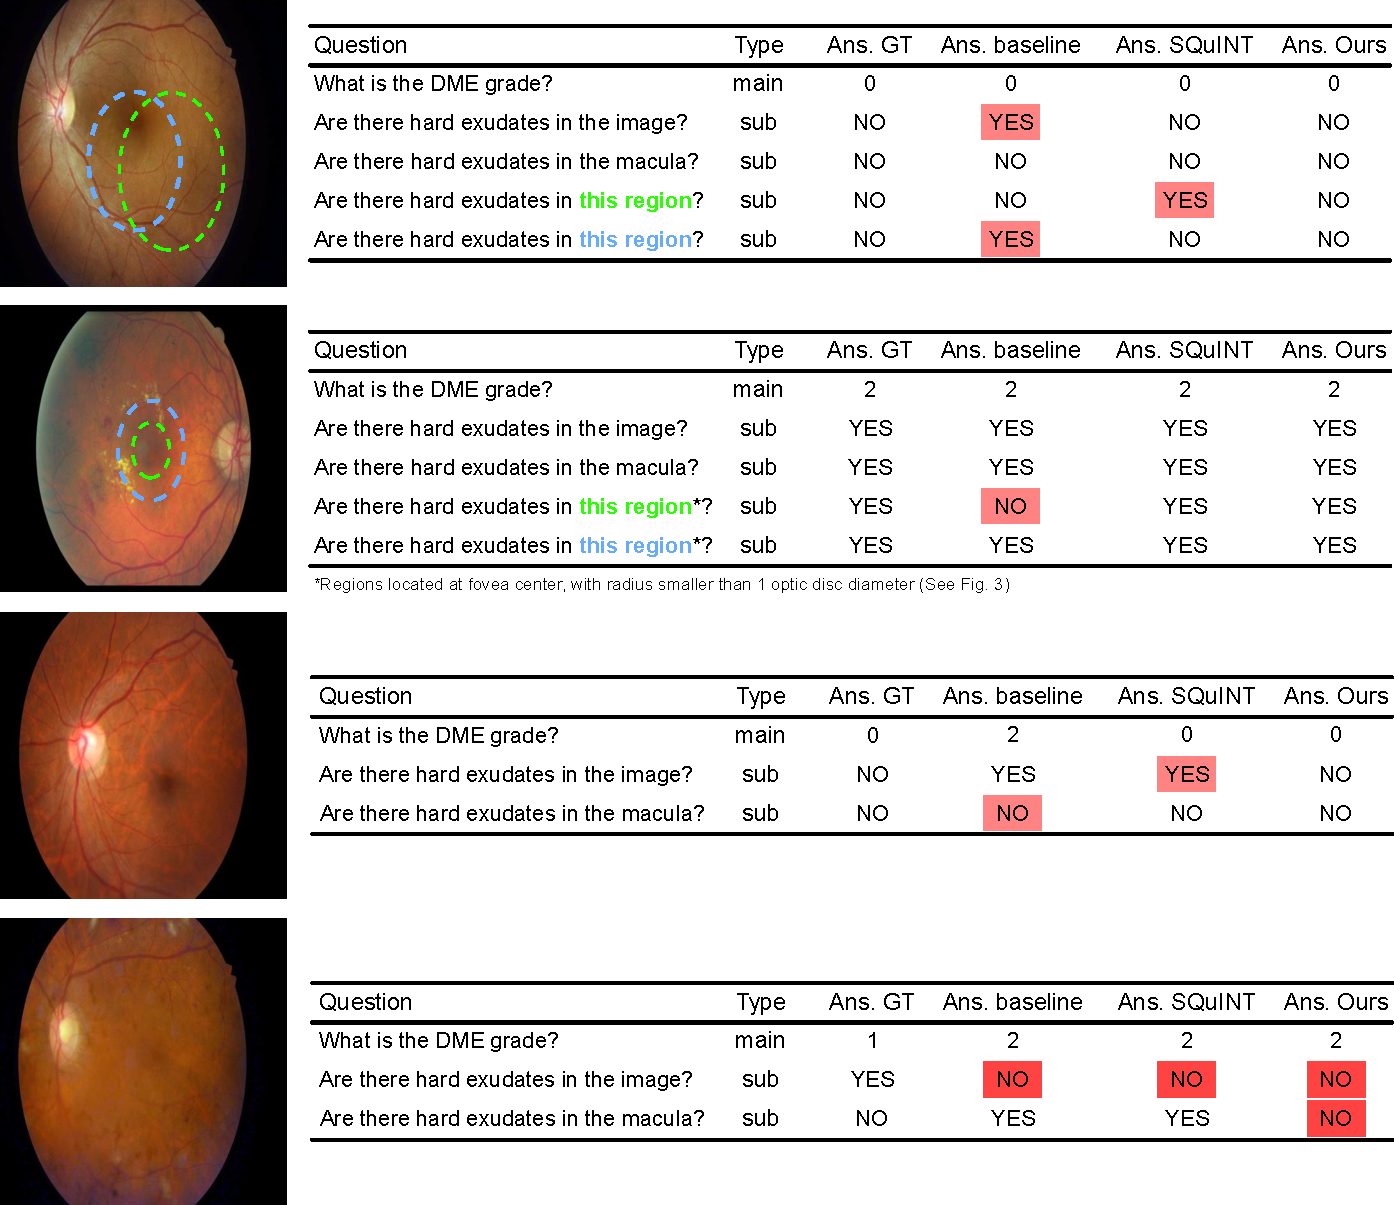
\includegraphics[width=0.99\textwidth]{Figures/Part2_Consist/01_mainsub/examples_expl_marked_add.pdf}
\caption{Qualitative examples from the test set. Inconsistent sub-answers are highlighted in red. Additional examples are shown in Appendix~\ref{appendix:consistency_mainsub}.  
}
\label{fig:examples}
\end{center}
\end{figure}


\begin{table}[!t]
\begin{center}
\begingroup
\setlength{\tabcolsep}{10pt} % Default value: 6pt
\renewcommand{\arraystretch}{1.5} % Default value: 1
\begin{tabular}{lllllllll}
\toprule
 \multicolumn{1}{c}{\multirow{2}{*}{$\lambda$}} & \multicolumn{1}{c}{\multirow{2}{*}{$\gamma$}} & \multicolumn{5}{c}{Accuracy}   & \multicolumn{2}{c}{Consistency}  \\ \cline{3-9} 
\multicolumn{1}{c}{}                         & \multicolumn{1}{c}{}      &  \multicolumn{1}{c}{overall}                       & \multicolumn{1}{c}{grade}      & \multicolumn{1}{c}{whole}        & \multicolumn{1}{c}{macula}        & \multicolumn{1}{c}{region}     & \multicolumn{1}{c}{C1}            & \multicolumn{1}{c}{C2}          
\\ \hline

\multicolumn{1}{l}{0}                     & \multicolumn{1}{l}{-}                    & \multicolumn{1}{l}{81.46} & \multicolumn{1}{l}{80.23} & \multicolumn{1}{l}{83.13} & \multicolumn{1}{l}{87.18} & \multicolumn{1}{l}{80.58} & \multicolumn{1}{l}{89.21} & \multicolumn{1}{l}{96.92} 

\\ \hline 

\multicolumn{1}{l}{0.2}                     & \multicolumn{1}{l}{0.5}                    & \multicolumn{1}{l}{82.01} & \multicolumn{1}{l}{80.38} & \multicolumn{1}{l}{83.59} & \multicolumn{1}{l}{86.56} & \multicolumn{1}{l}{81.36} & \multicolumn{1}{l}{90.93} & \multicolumn{1}{l}{97.38} 

\\ 
\multicolumn{1}{l}{0.2}                     & \multicolumn{1}{l}{1}                    & \multicolumn{1}{l}{82.65} & \multicolumn{1}{l}{ 79.77} & \multicolumn{1}{l}{ 83.97} & \multicolumn{1}{l}{ 86.64} & \multicolumn{1}{l}{82.30} & \multicolumn{1}{l}{ 93.22} & \multicolumn{1}{l}{97.51 } 

\\ 

\multicolumn{1}{l}{0.2}                     & \multicolumn{1}{l}{1.5}                    & \multicolumn{1}{l}{83.05} & \multicolumn{1}{l}{81.22} & \multicolumn{1}{l}{ 84.27} & \multicolumn{1}{l}{ 87.33} & \multicolumn{1}{l}{82.53} & \multicolumn{1}{l}{ 93.23} & \multicolumn{1}{l}{ 97.56} 


\\ \hline 
\multicolumn{1}{l}{0.3}                     & \multicolumn{1}{l}{0.5}                   & \multicolumn{1}{l}{82.34} & \multicolumn{1}{l}{ 79.92} & \multicolumn{1}{l}{ 83.59} & \multicolumn{1}{l}{ 87.71} & \multicolumn{1}{l}{81.74} & \multicolumn{1}{l}{ 92.32} & \multicolumn{1}{l}{ 97.31} 

\\ 

\multicolumn{1}{l}{0.3}                     & \multicolumn{1}{l}{1}                 & \multicolumn{1}{l}{83.27} & \multicolumn{1}{l}{ 80.53} & \multicolumn{1}{l}{ 84.58} & \multicolumn{1}{l}{ 87.25} & \multicolumn{1}{l}{82.91} & \multicolumn{1}{l}{ 94.01} & \multicolumn{1}{l}{ 98.10} 

\\ 

\multicolumn{1}{l}{0.3}                     & \multicolumn{1}{l}{1.5}                   & \multicolumn{1}{l}{83.28} & \multicolumn{1}{l}{80.84 } & \multicolumn{1}{l}{ 84.43} & \multicolumn{1}{l}{ 87.48} & \multicolumn{1}{l}{82.86} & \multicolumn{1}{l}{ 93.28} & \multicolumn{1}{l}{ 98.29} 


\\ \hline 

\multicolumn{1}{l}{0.4}                     & \multicolumn{1}{l}{0.5}                   & \multicolumn{1}{l}{82.87} & \multicolumn{1}{l}{80.69} & \multicolumn{1}{l}{ 84.89} & \multicolumn{1}{l}{ 87.02} & \multicolumn{1}{l}{82.30} & \multicolumn{1}{l}{ 92.66} & \multicolumn{1}{l}{ 96.66} 

\\ 
\multicolumn{1}{l}{0.4}                     & \multicolumn{1}{l}{1}                 & \multicolumn{1}{l}{82.97} & \multicolumn{1}{l}{ 80.15} & \multicolumn{1}{l}{ 83.97} & \multicolumn{1}{l}{ 86.72} & \multicolumn{1}{l}{82.69} & \multicolumn{1}{l}{ 93.91} & \multicolumn{1}{l}{98.23} 

\\ 
\multicolumn{1}{l}{0.4}                     & \multicolumn{1}{l}{1.5}                  & \multicolumn{1}{l}{83.33} & \multicolumn{1}{l}{ 80.08} & \multicolumn{1}{l}{ 84.20} & \multicolumn{1}{l}{ 86.87} & \multicolumn{1}{l}{83.17} & \multicolumn{1}{l}{ 93.96} & \multicolumn{1}{l}{ 97.77} 

\\ \hline 
\multicolumn{1}{l}{0.5}                     & \multicolumn{1}{l}{0.5}                & \multicolumn{1}{l}{82.54} & \multicolumn{1}{l}{81.07 } & \multicolumn{1}{l}{ 83.66} & \multicolumn{1}{l}{ 88.02} & \multicolumn{1}{l}{81.81} & \multicolumn{1}{l}{ 91.87} & \multicolumn{1}{l}{ 97.73} 

\\ 
\multicolumn{1}{l}{0.5}                     & \multicolumn{1}{l}{1}                    & \multicolumn{1}{l}{83.49} & \multicolumn{1}{l}{80.69 } & \multicolumn{1}{l}{84.96 } & \multicolumn{1}{l}{87.18} & \multicolumn{1}{l}{83.16} & \multicolumn{1}{l}{94.20} & \multicolumn{1}{l}{98.12 } 

\\ 
\multicolumn{1}{l}{0.5}                     & \multicolumn{1}{l}{1.5}             & \multicolumn{1}{l}{83.25} & \multicolumn{1}{l}{ 79.92} & \multicolumn{1}{l}{ 84.58} & \multicolumn{1}{l}{ 86.95} & \multicolumn{1}{l}{83.01} & \multicolumn{1}{l}{ 94.20} & \multicolumn{1}{l}{ 98.12} 

\\ \bottomrule                  
\end{tabular}
\endgroup
\end{center}
\caption{Average test accuracy and consistency values for different values of the parameters $\lambda$ and $\gamma$. The first row ($\lambda\, =\, 0$) corresponds to no consistency enhancement method.}
\label{tab:results_params}
\end{table}
In general, we observe that our proposed approach yields increases in accuracy and consistency when compared to both the baseline and SQuINT. Importantly, this increase in consistency is not at the expense of overall accuracy. Specifically, this indicates that our loss term causes the model to be correct about sub-questions when it is correct about main questions. The observed increase in accuracy also indicates that our approach is not synthetically increasing consistency by reducing the number of correct answers on main questions~\cite{selvaraju2020squinting}. We note that SQuINT results in a reduction in accuracy and consistency, which can be partially explained by the presence of region questions that are not associated to any main question. These questions, which exceed the number of main questions, may affect the constraint in the learned attention maps.

Table~\ref{tab:results_params} shows the effect of $\lambda$ and $\gamma$ on the performance metrics. As expected, we notice that when $\lambda$ increases, the consistency of our approach increases as well and will occasionally deteriorate overall accuracy. The impact of $\gamma$ however is less evident, as no clear trend is visible. This would imply that the exact parameter value used is moderately critical to performances. 